\section{Theorie}
Bei der Kernspinresonanz handelt es sich um einen Effekt der auftritt, da sich
die magnetischen Momente der Probenatomkerne in einem äußeren Magnetfeld
teilweise ausrichten.
Die entstehende Magnetisierung wird bei ausbleiben des äußeren Feldes
wieder gegen den Ausgangszustand streben und aus dem zeitlichen Verlauf der
Magnetisierung können Rückschlüsse auf Vorgänge innerhalb der Probe
und den Relaxationsvorgang an sich gezogen werden.
Hier können insbesondere Diffusion von magnetischen Momenten, Viskositäten und
Molekülradien untersucht werden.

\subsection{Magnetisierung im thermischen Gleichgewicht}
Wird eine Probe in ein äußeres Magnetfeld $B_{0}$ gebracht, so spalten die feldfreien Kernspinzustände $I$
in $2I+1$ Unterniveaus auf.
Der Energieunterschied zwischen zwei Niveaus beträgt jeweils $\gamma B_{0} \hbar$,
wobei $\gamma$ das gyromagnetische Verhältnis des Kerns und $\hbar$ das reduzierte Plancksche
Wirkungsquantum bezeichnen.
Nach der Boltzmannverteilung bildet sich zwischen zwei benachbarten Energieniveaus
$m$ und $m-1$ bei Temperatur $T$ ein Besetzungszahlverhältnis von
\begin{equation}
  \frac{N(m)}{N(m-1)} = \symup{e}^{-\frac{\gamma B_{0} \hbar}{kT}},
\end{equation}
$k$ bezeichnet hier die Boltzmannkonstante.
Es zeigt sich daher sofort, dass alle möglichen Energieniveaus unterschiedlich
stark besetzt sind.
Da ein Energieniveau zu einer Kernspinorientierung korrespondiert, liegt daher eine
Kernspinpolarisation vor.
Zusammen mit den magnetischen Momenten der Kernspins folgt daher ein magnetisches
Moment, dessen Betrag sich bei hinreichend kleinen äußeren Feldern im thermischen
Gleichgewicht mit der Vakuumpermeabilität $\mu_{0}$ zu
\begin{equation}
		M_0 = N \frac{\mu_0 \gamma^2 \hbar^2 B_0}{4 kT}
\end{equation}
berechnen lässt.
Die Größe $N$ bezeichnet hier die Anzahl der Momente pro Volumeneinheit und liegt
typischerweise in der Größenordnung \SI{e28}{\per\m}.

\subsection{Larmor-Präzession}
Die Gesamtmagnetisierung $\vec{M}$ der Probe entsteht durch das Zusammenspiel aller
Einzellmomente. Es handelt sich daher um eine makroskopische Größe, was die klassische
Berechnung rechtfertigt.
Da zum Auftreten einer Kernspinpolarisation ein äußeres Magnetfeld $\vec{B}$ angelegt werden muss,
wirkt ein Drehmoment
\begin{equation}
		\vec{D} = \vec{M} \times \vec{B} = \frac{\text{d} \vec{I}}{\text{d}t}
\end{equation}
auf $\vec{M}$ und es kommt zu einer Änderung des Gesamtdrehimpulses $\vec{I}$.
Weiterhin existiert ein Zusammenhang, der $\vec{M}$ und $\vec{I}$ über $\gamma$
koppelt, sodass sich bei Wahl des Magnetfeldes entlang der $z$-Richtung ein Differentialgleichungssystem
für die Komponenten der Magnetisierung
\begin{equation}
		\frac{\text{d} \vec{M_\text{z}}}{\text{d}t} = 0 ,  \hspace{1em}
		\frac{\text{d} \vec{M_\text{x}}}{\text{d}t} = \gamma \text{B}_0
		M_\text{y}, \hspace{1em}
		\frac{\text{d} \vec{M_\text{y}}}{\text{d}t} = \gamma \text{B}_0
		M_\text{x},
\end{equation}
ergibt.
Die Magnetisierung entlang der Feldrichtung ist trivialerweise konstant, sodass
die Magnetisierung eine Präzessionsbewegung die $z$-Achse
ausführt.
Diese Bewegung mit Frequenz
\begin{equation}
  \omega_{\text{L}} = \gamma B_{0}
\end{equation}
wird Larmor-Präzession genannt.

\subsection{Relaxationserscheinungen}
Wird die Magnetisierung nun durch Einstrahlung eines Hochfrequenzfeldes
aus der Gleichgewichtslage entfernt, so strebt sie nach der Anregung in einer Zeit $T_{i}$
wieder gegen ihre Gleichgewichtslage $\vec{M_{0}}$, sie relaxiert also.
Dieser Vorgang wird durch die Blochschen Gleichungen
\begin{align}
		\frac{\text{d} M_\text{z}}{\text{d} t} &= \frac{M_0 - M_\text{z}}{T_1} \\
		\frac{\text{d} M_\text{x}}{\text{d} t} &= \gamma B_0 M_\text{y} -
		\frac{M_\text{x}}{T_2} \\
		\frac{\text{d} M_\text{y}}{\text{d} t} &= \gamma B_0 M_\text{x} - \frac{M_\text{y}}{T_2}
\end{align}
beschrieben.
Es existieren zwei Arten an Relaxationsvorgängen:
\begin{itemize}
		\item \textbf{Spin-Gitter-Relaxationszeit/longitudinal ($T_{1}$):}
				Relaxationszeit parallel zur Feldrichtung. Gibt die Zeit
				an, die es dauert bis die Energie aus dem Spinsystem in Gitterschwingungen
				übergegangen ist.
		\item \textbf{Spin-Spin-Relaxationszeit/transversal ($T_{2}$):} Relaxationszeit
				unter anderem aufgrund der Spin Wechselwirkung von nächsten
				Nachbarn, als auch Feldinhomogenitäten. Auch hier können Spin-Gitter-Prozesse
        auftreten. Abnahme der zum $B$-Feld senkrechten Komponente.
\end{itemize}

\subsection{HF-Einstrahlvorgänge}
Wie bereits erwähnt, kann eine Magnetisierung durch Einstrahlung von Hochfrequenzfeldern
aus ihrer Gleichgewichtslage entfernt werden.
Der magnetische Feldvektor $\vec{B}_{1}$
des HF-Feldes soll dabei zu jeder Zeit senkrecht zur vorher gewählten
Magnetfeldrichtung stehen, das Hochfrequenzfeld verhält sich daher wie
\begin{equation}
  \vec{B}_{\text{HF}} = 2 \vec{B}_{1} \cos{(\omega t)}.
\end{equation}
Bei Übergang in ein mitbewegtes Koordinatensystem zeigt sich, dass die Magnetisierung
durch die Präzession des Magnetisierungsvektors um das effektive Magnetfeld
\begin{equation}
  \vec{B}_{\text{eff}} = \vec{B}_{0} + \vec{B}_{1} + \frac{\vec{\omega}}{\gamma}
\end{equation}
beschrieben wird.
Im Fall, dass die Frequenz des HF-Feldes der Larmorfrequenz entspricht,
Fallen $\vec{B}_{\text{eff}}$ und $\vec{B}_{1}$ genau aufeinander.
Die Präzessionsbewegung findet also auf einem Kegel mit Öffnungswinkel \SI{90}{\degree} statt.
Durch Steuerung der Einstrahlzeit der HF-Pulse kann $\vec{M}$ um einen beliebigen
Winkel gedreht werden.
So dreht
\begin{equation}
		\symup{\Delta} t_{90} = \frac{\pi}{2 \gamma B_1}
\end{equation}
$\vec{M}$ aus $z$- in $y$-Richtung, die doppelte Zeit $ 2 \symup{\Delta} t_{90} =  \symup{\Delta} t_{180}$
aus der $z$- in die $-z$-Richtung.

\subsection{Einfluss der Diffusion auf das Relaxationsverhalten einer flüssigen Probe}
Da das Verhalten der Probe nicht statisch ist, wird die Larmorfrequenz zeitabhängig.
Durch zwangsweise vorkommende Inhomogenitäten des B-Feldes und Diffusion von Kernspins
durch die Brownsche Molekularbewegung spüren einzelne Spins zeitabhängig ein
sich veränderndes Magnetfeld.
Dadurch resultiert, dass die Amplitude der Magnetisierung schneller abnimmt, als
durch die Blochschen Gleichungen beschrieben, sie müssen also modifiziert werden.
Durch Erweiterung um einen Term
\begin{equation}
		\frac{\partial M}{\partial t} = D \Delta \vec{M}
\end{equation}
mit Diffusionskonstante D wird die Lösung der Magnetisierungsbewegung zu
\begin{equation}
		M_\text{tr} = f(x,y,z,t) \cdot \exp(-i\omega_\text{L}t) \cdot
		\exp\left(-\frac{t}{T_\text{2}}\right),
\end{equation}
wobei die Funktion $f$ mit dem Feldgradienten $G$ dem Zusammenhang
\begin{equation}
		\frac{\partial f}{\partial t} = \left(-i \gamma Gz + D \Delta \right) f
\end{equation}
gehorcht.
Der erste Summand beschreibt hierbei eine Präzessionsbewegung, der zweite eine
Diffusion.
Wird die Probe nun mehreren $\symup{\Delta} t_{180}$-Pulsen ausgesetzt, was die
Grundlage vieler Messmethoden ist, lässt sich die Magnetisierungsamplitude durch
\begin{equation}
		M_\text{y}(t) = M_0 \exp \left( - \frac{t}{T_2} \right) \exp \left( -
		\frac{t}{T_\text{D}} \right)
\end{equation}
beschreiben.
Hierbei muss die Diffusionsrelaxationszeit $T_{\text{D}}$ möglichst groß gewählt werden,
damit die Relaxationszeit $T_{2}$ gemessen werden kann.
Dies ist möglich, da
\begin{equation}
  T_\text{D} = \frac{3}{D \gamma^2 G^2 \tau^2}
\end{equation}
gilt.
Die Größe $\tau$ beschreibt dabei den halben zeitlichen Abstand zwischen zwei
$\symup{\Delta} t_{180}$-Pulsen und ist prinzipiell frei wählbar, wodurch sich
die Diffusionsrelaxationszeit einstellen lässt.

\section{Messverfahren und Aufbau}
\subsection{Aufbau}
\autoref{Theo:Abb_1} zeigt den prinzipiellen Aufbau der verwendeten Apparatur.
Die Probe ist dabei zwischen zwei Polschuhen gelagert, zwischen denen ein Magnetfeld
erzeugt wird.
Senkrecht zu den Polschuhen kann das HF-Magnetfeld angelegt werden.
Zur Messung der Relaxationszeiten wird die Induktionsspannung entlang der
$xy$-Ebene gemessen.
Die verwendete Apparatur ist fertig aufgebaut und bedarf lediglich einer
vorherigen Justage.

\begin{figure}[h]
		\centering
		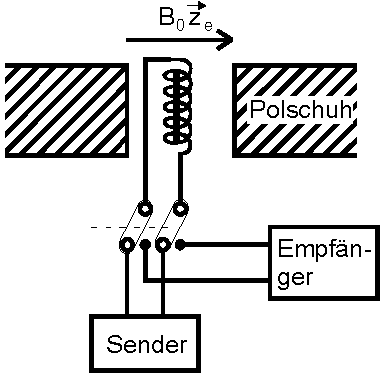
\includegraphics[width=0.3\linewidth]{content/pics/aufbau.pdf}
		\caption{Schematischer Aufbau zur Vermessung der Kernspinresonanz\cite{anleitung}. }
		\label{Theo:Abb_1}
\end{figure}

\subsection{Freier Induktionszerfall (FID)}
Wird die Probe einem $\symup{\Delta} t_{90}$-Puls ausgesetzt, wird die Magnetisierung in
die $xy$-Ebene gebracht und beginnt dort zu präzedieren.
Mit der Zeit relaxiert die Magnetisierung wieder in die Gleichgewichtslage, da es
zu Wechselwirkungen mit Nachbarn und Feldinhomogenitäten kommt und es kommt zu einer
Dephasierung der Spins entlang der $z$-Achse.
Für hinreichend homogene Felder kann die Relaxationszeit
\begin{equation}
		\frac{1}{T_2^*} = \frac{1}{T_2} + \frac{1}{T_{\Delta B}}
\end{equation}
gemessen werden, der Signalverlauf ist im Zeitraum $0$ bis $\tau$ in \autoref{Theo:Abb2}
gezeigt.

\subsection{Spin-Echo-Verfahren}
Um trotz der Feldinhomogenitäten eine Relaxationszeit messen zu können, kann
das Spin-Echo-Verfahren angewendet werden.
Hierbei wird am Ende des FID zur Zeit $\tau$, wenn alle Spins dephasiert sind und daher kein Signal
mehr messbar ist, ein $\symup{\Delta} t_{180}$-Puls auf die Probe gegeben.
Als Resultat laufen die dephasierenden Spins zum Zeitpunkt $2\tau$
wieder zusammen und es entsteht ein Signal mit umgekehrten Vorzeichen und niedrigerer Amplitude
\begin{equation}
		M_\text{y}(t) = M_0 \exp\left(-\frac{t}{T_2} \right)s.
\end{equation}
Aus der exponentiellen Abnahme der Amplituden lässt sich so die Relaxationszeit bestimmen,
der Signalverlauf ist wieder in \autoref{Theo:Abb2} zu sehen.

\begin{figure}[h]
		\centering
		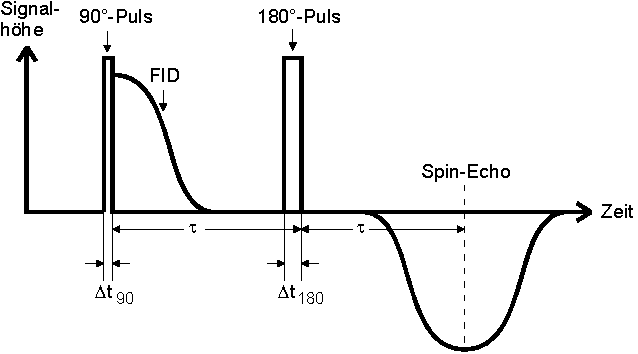
\includegraphics[width=0.8\linewidth]{content/pics/signalverlauf.pdf}
		\caption{Signalverlauf in Abhängigkeit der Zeit bei dem
		Spin-Echo-Verfahren \cite{anleitung}.}
		\label{Theo:Abb2}
\end{figure}

\subsection{Carr-Purcell- und Meibooms-Gill-Methode}
Nachteilig an der Spin-Echo-Methode ist die lange Wartezeit, da mit einer neuen
Messung gewartet werden muss, bis sich die Gleichgewichtslage wieder eingestellt hat.
Hier bietet es sich an, gleich mehrere $\symup{\Delta} t_{180}$-Pulse in gleichen
Abständen $2\tau$ auf die Probe zu geben, sodass eine ganze Reihe von Spin-Echos
aufgenommen werden kann.
Problematisch ist hierbei, dass die nicht vermeidbaren Justagefehler bei der Dauer
der $\symup{\Delta} t_{180}$-Pulse dazu führen, dass die Magnetisierung mit steigender
Zahl der Pulse immer weiter von der $xy$-Ebene abweichen.
Dieses Problem bei der Carr-Purcell-Methode kann durch die Meibooms-Gill-Methode
ausgeglichen werden.
Durch eine spezielle Vorrichtung wird die Phase der $\symup{\Delta} t_{180}$-Pulse
um \SI{90}{\degree} gegenüber dem $\symup{\Delta} t_{90}$-Puls gedreht.
Für geradzahlige Echos kompensieren sich die Fehler gerade und die Amplituden
haben den richtigen Wert.

\subsection{Methode zur Bestimmung der Spin-Gitter-Relaxationszeit}
Die Bestimmung von $T_{1}$ ist ungemein einfacher als die für $T_{2}$.
Hierfür wird die Magnetisierung zuerst mit einem $\symup{\Delta} t_{180}$-Puls
in $-z$-Richtung gekippt.
Nach einer Zeit $\tau$ wird ein $\symup{\Delta} t_{90}$ Impuls gegeben und die restliche
Amplitude gemessen.
Mit den Anfangsbedingungen $M_x(0) = M_y(0) =0 \text{ und } M_z(0)=-M_0$
geben die Blochschen Gleichungen für die Amplitude
\begin{equation}
		M_\text{z}(\tau) = M_0 \left(1 - 2 \exp \left(- \frac{\tau}{T_1} \right)
		\right)
\end{equation}
und die Relaxationszeit kann aus der Abhängigkeit zwischen $M_{\text{z}}$ und $\tau$
bestimmt werden.

\subsection{Viskositätsmessung}
Zur Viskositätsmessung wird ein Kapillar-Viskosimeter eingesetzt.
Die zu vermessende Flüssigkeit läuft dabei über eine Kapillare ab, die Geschwindigkeit
des Vorgangs wird durch die Viskosität bestimmt.
Da die Viskosität der Flüssigkeit proportional zur Abflussgeschwindigkeit ist,
lässt sich diese bestimmen.
Dazu wird die Zeit gemessen, in der die Flüssigkeit zwischen zwei Markierungen steht.

\section{Durchführung}
\subsection{Justage}
Zur Justage wird eine Lösung von paramagnetischem Kupfersulfat in Wasser als
Probe eingebracht.
Es werden daraufhin die FID-Parameter Larmorfrequenz, Shim und Pulslänge auf
maximale Amplitude und minimale Zerfallsdauer eingestellt.
Um Überschwinger zu unterdrücken muss die Wiederholungszeit auf \SI{15}{\second}
eingestellt werden.
Nach erfolgreicher Justage wird die Probe durch bidestiliertes Wasser ersetzt und
die Parameter abschließend überprüft.

\subsection{Bestimmung der Relaxationszeiten}
Zur Bestimmung der Spin-Gitter-Relaxationszeit werden die
Pulslängen A und B auf einen $\symup{\Delta} t_{180}$- und einen
$\symup{\Delta} t_{90}$-Puls eingestellt.
Über ein Oszilloskop können die Maxima des zweiten Impulses abgelesen werden.
Es werden mehrere Messwerte für verschiedene Abstände $\tau$ aufgenommen.
Danach wir die Apparatur auf die Meiboom-Gill-Methode (Schalter MG) gestellt.
Bei möglichst kleinen Abständen $\tau$ wird nun eine Reihe von Spin-Echos erzeugt
und das Bild ausgelesen.
Abschließend wird eine Aufnahme eines Bildes nach der Carr-Purcell-Methode
gemacht.

\subsection{Messung der Diffusionskonstante und des Molekülradius}
Bei möglichst konstanter Temperatur und maximalem Feldgradienten wird die
Zeit variiert, in der der $\symup{\Delta} t_{180}$-Puls gegeben wird
und die Amplitude der Spin-Echos gemessen.
Der Feldgradient kann dabei aus der Halbwertsbreite der Spin-Echos bestimmt werden.
Die Bestimmung des Molekülradius kann aus der Diffusionskonstante geschehen, dazu
ist jedoch die Kenntnis der Viskosität notwendig.
Diese wird mittels eines Kapillar-Viskosimeters bestimmt.
